\documentclass[11pt,letterpaper]{article}

\usepackage[utf8]{inputenc}
\usepackage[spanish]{babel}
\usepackage{float}
\usepackage{xcolor}
\usepackage{verbatim}
\usepackage{mwe}
\usepackage{charter}
\usepackage{afterpage}
\usepackage{amsmath}
\usepackage{appendix}
\usepackage{ragged2e}
\usepackage{array}
\usepackage{etoolbox}
\usepackage{fancyhdr}
\usepackage{booktabs}
\usepackage{arydshln}
\usepackage[justification=justified,singlelinecheck=false,labelfont=bf,format=plain]{caption}
\usepackage[justification=justified,singlelinecheck=false,labelfont=bf,format=plain]{subcaption}
\usepackage{enumitem}
\usepackage[bottom=2.5cm,top=2.0cm,left=2.0cm,right=2.0cm]{geometry}
\usepackage{graphicx}
\usepackage{indentfirst}
\usepackage{mathtools}
\usepackage{multirow}
\usepackage{pdfpages}

\usepackage{subfiles}
\usepackage[compact]{titlesec}
\usepackage{blindtext}
\usepackage{stfloats}
\usepackage{lipsum} 


\renewcommand{\familydefault}{\rmdefault}

\newcommand\blankpage{
    \null
    \thispagestyle{empty}
    \addtocounter{page}{0}
    \newpage}
    \title{Circuito RC con salida en C respuesta escalón}
    \author{Álvaro Martín Romero}
\begin{document}
\maketitle	
\section{Simulación del circuito}%
\label{sec:Simulación del circuito}
Para este circuito necesitamos los siguientes materiales:
\begin{itemize}
	\item Fuente de alimentación
	\item Osciloscopio Tektronix TPS2012
	\item Generador de Funciones Tektronix AGF3000
	\item Inductancia 350mH
	\item Resistencia 10 K$\Omega$
\end{itemize}
Se adjunta a continuación el circuito RC con salida en C en escalón simulado en MultisimLive:
\begin{figure}[H]
	\centering
	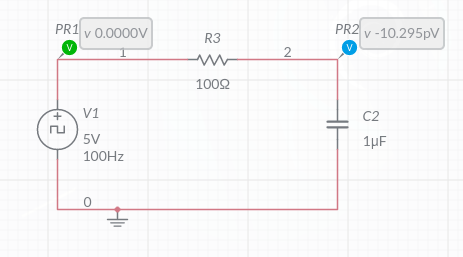
\includegraphics[width=0.8\textwidth]{imagen/circuitoRL_Rescalon.png}
	\caption{Circuito RC con salida en C con escalón simulado en el programa MultisimLive}
	\label{fig:imagen-circuitoRL}
\end{figure}
\section{Estudio del circuito RL}%
\label{sec:Estudio del circuito RL}
Para calcular el voltaje de salida en función del de entrada, primero necesitamos conocer cuanto vale la función de transferencia. Esta sabemos que es:
\[
	G\left( s \right) =\frac{V_s(s)}{V_e(s)}
.\] 
Con los valores de tensión de salida y de entrada dados por $V_s\left( s \right) =\frac{I}{Cs}$ y $V_e\left( s \right) =I\left( R+\frac{1}{Cs} \right) $. Por tanto
\[
	G\left( s \right) =\frac{1}{R+s}
.\] 
donde \[
	T=RC
.\] 
La respuesta temporal del circuito es $Y(s)=G(s)\cdot R(s)$ donde $R(s)$ es la transformada de Laplace en la entrada. Desarrollando esa función con nuestro caso y aplicando transformaciones inversas de Laplace se llega a que:
\[
	V_{s}=V_e\cdot \left(1-e^{-\frac{t}{T}} \right) 
.\] 

En nuestro circuito, $T=R\cdot C=100 \Omega \cdot 1 \mu F= 0.0001 s$, $V_e= 5 V$ y $t=20\mu s$ por tanto:
\begin{equation}
	\boxed{V_s=0.906V}
\end{equation}
\section{Simulación del circuito}%
\label{sec:Simulación del circuito}
Simulamos ahora el circuito visto en la figura (1):
\begin{figure}[H]
	\centering
	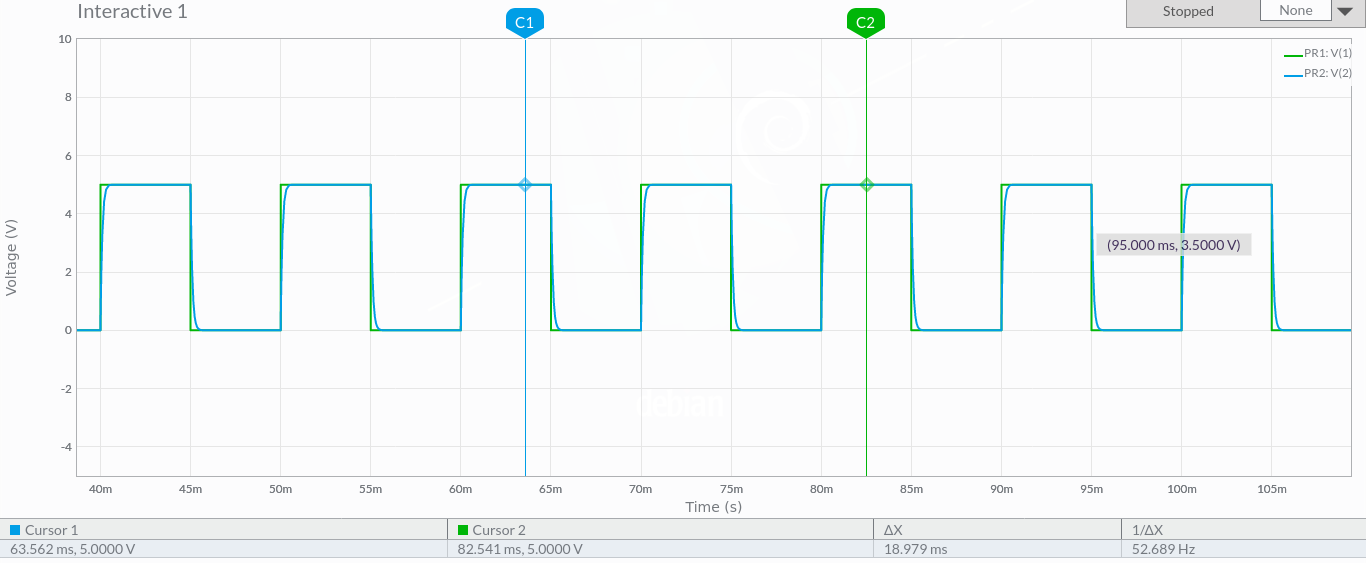
\includegraphics[width=0.8\textwidth]{imagen/analisisRL_R_escalongrande.png}
	\caption{Representación gráfica hecha gracias al simulador donde podemos observar la forma escalonada que genera la fuente.}
	\label{fig:imagen-analisisRL_R_escalongrande-png}
\end{figure}
Como vemos en la imagen anterior, observamos la forma escalonada que genera la fuente, sin embargo, esto no nos da nada de información acerca de la tensión de salida que queremos medir experimentalmente, para ello haremos zoom a la zona donde empieza a verse los efectos exponenciales de la tensión de salida:
\begin{figure}[H]
	\centering
	\includegraphics[width=0.8\textwidth]{imagen/analisisRL_Rescalonpequeño.png}
	\caption{Representación gráfica ampliada donde se puede observar el comportamiento exponencial de la tensión de salida}
	\label{fig:imagen-analisisRL_Rescalonpeque-png}
\end{figure}
Aquí podemos observar el comportamiento exponencial de la tensión de salida, donde el cursor de color azul marca el valor de $t=20\mu s$, cuyo valor de la tensión es igual que el valor teórico esperado
\end{document}
